	\section*{27/09}
	\begin{center}
		\textbf{Одномерные краевые задачи}
	\end{center}
	\begin{equation}\label{eq}
		- (ku')' + cu' + bu = f, \qquad x \in (0, l),
	\end{equation}	
	
	где $u(x)$ - неизвестная функция; $k(x), \ c(x), \ b(x), \ f(x)$ - известные функции.
	
	 \begin{table}[ht]
	 \centering
	 \caption{Граничные условия}
	 \label{cond}
	 \begin{tabular}{| c | c | c | p{10cm}|}
		\hline
		№ &x = 0 & x = l  \\
		\hline
		1& $u(0) = U_0$ & $u(l) = U_l$ \\
		\hline
		2& $k(0)u'(0) = - \sigma_0$ & $k(l)u'(l) = \sigma_l$ \\
		\hline
		3& $k(0)u'(0) = -a_0(U_0 - u(0))$ & $k(l)u'(l) = a_l(U_l - u(l))$ \\
		\hline
	\end{tabular}
	\end{table}
	
	\begin{center}
		\textbf{Интегральная формулировка}
	\end{center}
	
	Состасим невязку:
	\begin{equation} \label{discrepancy}
	r = -(ku')' + cu' + bu - f = 0
	\end{equation}
	
	\eqref{eq} $\Leftrightarrow$ \eqref{discrepancy}
	
	Составим следующий интеграл:
	\begin{equation} \label{int}
	\int \limits_0^l r \cdot v dx = 0,
	\end{equation}
	где $v$ -- некоторая пробная функция ($v = \delta u$ -- возможные изменения $u$)
	
	Докажем, что \eqref{int} $\Leftrightarrow$ \eqref{discrepancy}:
	
	Предположим, что \eqref{int} выполняется, а \eqref{discrepancy} -- нет, то есть $r \neq 0$. Тогда:
	
	$v$ -- любая пробная функция:
	
\begin{figure}[ht]
    \centering
    \begin{tikzpicture}
        \begin{axis}[
            title={Графики $r(x)$ и $v(x)$},
            xlabel={$x$},
            ylabel={$y$}, 
            ymin=-1, ymax=1,
            samples=300,
            xmin=0, xmax=2*pi,
            xtick={0, pi/2, pi, 3*pi/2, 2*pi},
            xticklabels={0,,,$l$,}, 
            ytick={0}, 
            yticklabels={0}, 
            grid=both,
            axis lines=middle,
            every axis line/.append style={->, thick}, 
            tick label style={font=\footnotesize} 
        ]
        \addplot[blue, thick] {sin(deg(x))}; 
        \addplot[red, thick] {sin(deg(x))/2}; 
        \legend{$r(x)$, $v(x)$} 
        \end{axis}
    \end{tikzpicture}
\end{figure}

\begin{figure}[ht]
    \centering
    \begin{tikzpicture}
        \begin{axis}[
            title={График $r(x) \cdot v(x)$},
            xlabel={$x$},
            ylabel={$y$}, 
            ymin=-1, ymax=1,
            xmin=0, xmax=2*pi,
            samples=300,
            xtick={0, pi/2, pi, 3*pi/2, 2*pi},
            xticklabels={0,,,$l$,}, 
            ytick={0}, 
            yticklabels={0}, 
            grid=both,
            axis lines=middle,
            every axis line/.append style={->, thick}, 
            tick label style={font=\footnotesize} 
        ]
        \addplot[blue, thick] {sin(deg(x)) * (sin(deg(x))/2)};
        \end{axis}
    \end{tikzpicture}
\end{figure}

\newpage
	
	Из последнего графика видно, что
	\[\int \limits_0^l r \cdot v dx \neq 0,\]
	
	что противоречит нашему предположению о том, что \eqref{int} выполняется, ч.т.д.

Итак,
\begin{equation}\label{int1}
	\int \limits_0^l r \cdot v dx = \int \limits_0^l (-(ku')' v+ cu' v+ buv - fv ) dx = 0
\end{equation}	

Интегрируем по частям первый интеграл:
\begin{equation}\label{int_part}
	\int \limits_0^l -(ku')' v dx = 
	\begin{vmatrix}
	\int \limits_0^l f dg = fg \bigg |_0^l - \int \limits_0^l g df \\
	dg = -(ku')'dx & g = -ku'\\
	f = v & df = v' dx
	\end{vmatrix} =
\end{equation}	
\[= -ku' v \bigg |_0^l + \int \limits_0^l (ku') v' dx = \int \limits_0^l (ku') v' dx - \underbrace{(\underbrace{k(l)u'(l)v(l)}_{F_l}  \underbrace{- k(0)u'(0)v(0)}_{F_0})}_{F(v)}\]

Подставим \eqref{int_part} в \eqref{int1}:
\[\int \limits_0^l ((ku')' v' + cu' v+ buv - fv ) dx - F(v) = 0\]

Рассмотрим граничные условия:
\begin{table}[ht]
	 \centering
	 \label{cond2}
	 \begin{tabular}{| c | c | c | p{10cm}|}
		\hline
		№ &x = 0 & x = l  \\
		\hline
		1& $u(0) = U_0 \Rightarrow v(0) = 0,\ F_0 = 0$ & $u(l) = U_l \Rightarrow v(l) = 0,\ F_l = 0$ \\
		\hline
		2& $k(0)u'(0) = - \sigma_0 \Rightarrow F_0 = \sigma_0 v(0)$ & $k(l)u'(l) = \sigma_l \Rightarrow F_l = \sigma_l v(l)$ \\
		\hline
		3& $k(0)u'(0) = -a_0(U_0 - u(0)) \Rightarrow$ & $k(l)u'(l) = a_l(U_l - u(l)) \Rightarrow$ \\
		& $\Rightarrow F_0 = a_0 (U_0 - u(0)) v(0)$ & $\Rightarrow F_l = a_l (U_l - u(l)) v(l)$ \\
		\hline
	\end{tabular}
	\end{table}
	
	Разобьем отрезок $[0, l]$ на части $[x_i, x_{i+1}]$:
\begin{center}
\begin{tikzpicture}
    \draw (0, 0) -- (9.5, 0);
    
    \draw (0, 0.1) -- (0, -0.1) node[below] {$x_{0} = 0$};
    \draw (1.5, 0.1) -- (1.5, -0.1) node[below] {$x_{1}$};
    \draw (4.2, 0.1) -- (4.2, -0.1) node[below] {$x_{i}$};
    \draw (5.7, 0.1) -- (5.7, -0.1) node[below] {$x_{i + 1}$};
    \draw (8, 0.1) -- (8, -0.1) node[below] {$x_{n-1}$};
    \draw (9.5, 0.1) -- (9.5, -0.1) node[below] {$x_{n} = l$};
    
    \node at (2.8, -0.4) {\dots};
    \node at (6.8, -0.4) {\dots};
    
    \node at (5, 0.4) {$i$};
    
    \draw[thin] (4.2, 0.5) -- (4.2, 0);
    \draw[->][thin] (4.2, 0.5) -- (3.2, 0.5) node[above] {$t_i^{(1)}$};
    
    \draw[thin] (5.7, 0.5) -- (5.7, 0);
    \draw[->][thin] (5.7, 0.5) -- (6.7, 0.5) node[above] {$t_i^{(2)}$};
\end{tikzpicture}
\end{center}
\begin{equation}\label{int_xi}
\int \limits_{x_i}^{x_{i+1}} r \cdot v dx = 0 \Rightarrow \int \limits_{x_i}^{x_{i+1}} [(ku')v' + cu'v + buv - fv] dx - t_1^{(i)}v_i - t_2^{(i)}v_{i+1} = 0,
\end{equation}

где $t_1^{(i)}, t_2^{(i)}$ -- реакции отброшенных сил
\[t_1^{(i)} = -k(x_i) u'(x_i) \qquad \qquad t_2^{(i)} = -k(x_{i+1}) u'(x_{i+1})\]
\[v_i = v(x_i) \qquad \qquad v_{i+1} = v(x_{i+1})\]

\[u = N_1^{(i)} u_i + N_2^{(i)} u_{i+1},\]

где $N_1^{(i)}, N_2^{(i)}$ -- полиномы Лагранжа:
\begin{center}
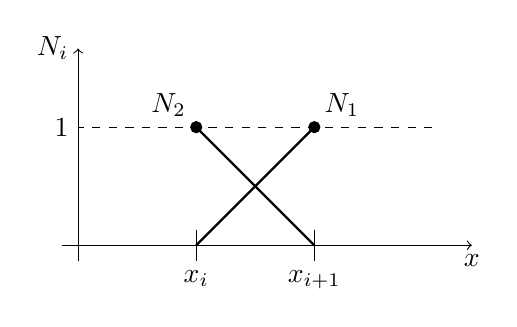
\begin{tikzpicture}
    \draw[->] (-0.2, 0) -- (5, 0) node[below] {$x$};
    \draw[->] (0, -0.2) -- (0, 2.5) node[left] {$N_i$};
    \draw[dashed] (4.5, 1.5) -- (0, 1.5) node[left] {1};
    \draw (1.5, 0.2) -- (1.5, -0.2) node[below] {$x_i$};
    \draw (3, 0.2) -- (3, -0.2) node[below] {$x_{i+1}$};
    \draw[thick] (1.5, 0) -- (3, 1.5) node[above right] {$N_1$};
    \draw[thick] (3, 0) -- (1.5, 1.5) node[above left] {$N_2$};
    \filldraw (3, 1.5) circle (2pt);
    \filldraw (1.5, 1.5) circle (2pt);
\end{tikzpicture}
\end{center}

Аппроксимируем неизвестную функцию $u$:
\[u = \alpha_1 + \alpha_2 x\]
\begin{center}
\begin{tikzpicture}
    \draw[->] (-0.2, 0) -- (5, 0) node[below] {$x$};
    \draw[->] (0, -0.2) -- (0, 3) node[left] {$u$};
    \draw (1.5, 0.2) -- (1.5, -0.2) node[below] {$x_i$};
    \draw (3, 0.2) -- (3, -0.2) node[below] {$x_{i+1}$};
    \draw[dashed] (1.5, 0) -- (1.5, 1);
    \draw[dashed] (1.5, 1) -- (0, 1) node[left] {$u_i$};
    \draw[dashed] (3, 2)--(3, 0);
    \draw[dashed] (3, 2) -- (0, 2) node[left] {$u_{i+1}$};
    \draw (1.5, 1) -- (3, 2);
    \filldraw (1.5, 1) circle (2pt);
    \filldraw (3, 2) circle (2pt);
\end{tikzpicture}
\end{center}
\[\begin{cases}
u(x_i) = \alpha_1 + \alpha_2 x_i = u_i\\
u(x_{i+1}) = \alpha_1 + \alpha_2 x_{i+1} = u_{i+1}
\end{cases}\]

Поиск коэффициентов $\alpha_1, \alpha_2$:
\[\Delta =
\begin{vmatrix}
1 & x_i \\
1 & x_{i+1}
\end{vmatrix} = x_{i+1} - x_i = l_i
\]
\[\Delta_1 =
\begin{vmatrix}
u_i & x_i \\
u_{i+1}  & x_{i+1}
\end{vmatrix} = u_ix_{i+1} - u_{i+1} x_i
\]
\[\Delta_2 =
\begin{vmatrix}
1 & u_i \\
1 & u_{i+1}
\end{vmatrix} = u_{i+1} - u_i
\]
\[\alpha_1 = \frac{u_ix_{i+1} - u_{i+1} x_i}{l_i},\ \ \alpha_2 = \frac{u_{i+1} - u_i}{l_i}\]

Подставляем в $u$:
\[u = \frac{u_ix_{i+1} - u_{i+1} x_i}{l_i} + \frac{u_{i+1} - u_i}{l_i} x = \underbrace{\left(\frac{x_{i+1} - x}{l_i} \right)}_{N_1^{(i)}} u_i + \underbrace{\left(\frac{x - x_i}{l_i} \right)}_{N_2^{(i)}} u_{i+1}\]

В матричном виде:
\[u = Nq,\ N = [ \underbrace{N_1^{(i)},\ \ N_2^{(i)}}_{\text{функции формы}}],\ q = 
\begin{bmatrix}
u_i \\
u_{i+1}
\end{bmatrix}
\]
\[N_1^{(i)} = \frac{x_{i+1} - x}{l_i} = 1 - \frac{x - x_i}{l_i}\]
\[N_2^{(i)} = \frac{x - x_i}{l_i}\]

Вернемся к интегралу \eqref{int_xi}:
\[u = Nq\]
\[u' = \frac{dN}{dx}q = Bq,\]

где $B$ -- матрица производных от функций форм:
\[B = \left[ -\frac{1}{l_i},\ \ \frac{1}{l_i} \right]\]
\[v = N \delta q,\ \ \delta q = [v_i\ \ v_{i+1}]\]
\[v' = B \delta q\]

Подставляем в \eqref{int_xi}:
\[\int \limits_{x_i}^{x_{i+1}} [ \underbrace{ (B \delta q)^T}_{(v')^T } k \underbrace{Bq}_{u' } + \underbrace{(N \delta q)^T}_{v^T } c \underbrace{Bq}_{u' } + \underbrace{(N \delta q)^T}_{v^T } b \underbrace{Nq}_{u } - \underbrace{(N \delta q)^T}_{v^T } f] dx-\]\[ - t_1^{(i)}v_i - t_2^{(i)}v_{i+1} = 0\]
\[\int \limits_{x_i}^{x_{i+1}}  \delta q^T [(B^T k B + N^T c B + N^T b N)q - N^T f] dx - t_1^{(i)}v_i - t_2^{(i)}v_{i+1} = 0\]
\[\int \limits_{x_i}^{x_{i+1}} (B^T k B + N^T c B + N^T b N )dx = K^{(i)}\]
\[\int \limits_{x_i}^{x_{i+1}} N^T f dx = P^{(i)}\]

$K^{(i)}$ и $P^{(i)}$ -- матрицы $2 \times 2$.
\[t_1^{(i)}v_i + t_2^{(i)}v_{i+1} = \delta q^T t^{(i)},\ \ t^{(i)} = 
\begin{bmatrix}
t_1^{(i)} \\
t_2^{(i)}
\end{bmatrix}
\]

$\delta q^T \neq 0$, поэтому можно сократить.

Получившаяся СЛАУ:
\[
\fcolorbox{red}{red!20}{$K^{(i)} q = P^{(i)} + t^{(i)}$}
\]




























